\documentclass[UTF8,11pt,a4paper]{ctexart}
\usepackage[a4paper,margin=2.15cm]{geometry}
\usepackage{amsmath,amssymb}
\usepackage{booktabs}
\usepackage{graphicx}
\usepackage{xcolor}
\usepackage{hyperref}
\usepackage[numbers,sort&compress]{natbib}
\usepackage{microtype}
\usepackage{enumitem}
\usepackage{fancyhdr}
\usepackage{array}
\usepackage{caption}
\usepackage{float}

\definecolor{RangerPurple}{HTML}{5A189A}
\definecolor{RangerGreen}{HTML}{2A9D8F}
\hypersetup{
  colorlinks=true,
  linkcolor=RangerPurple,
  citecolor=RangerGreen,
  urlcolor=RangerPurple,
  pdftitle={从数值优化到可复核证明：Heisenberg/XXZ 链热力学能量密度的对称分块机器认证},
  pdfauthor={Ranger Team}
}
\graphicspath{{figures/}}
\captionsetup{font=small,labelfont=bf}
\setlist{nosep,leftmargin=2em}
\setlength{\parindent}{2em}
\setlength{\parskip}{0.25em}
\pagestyle{fancy}
\fancyhf{}
\fancyhead[L]{Quantum Harness Challenge \#230}
\fancyhead[R]{Ranger Team}
\fancyfoot[C]{\thepage}
\setlength{\headheight}{14pt}

\newcommand{\cert}{\mathrm{cert}}
\newcommand{\eB}{e_{\mathrm B}}
\newcommand{\code}[1]{\texttt{#1}}

\title{
  \textbf{从数值优化到可复核证明}\\[0.45em]
  \large Heisenberg/XXZ 链热力学能量密度的对称分块机器认证
}
\author{Ranger Team\\Chenxi Wan \quad Yedi Shen \quad Junkai Wang}
\date{2026 年 7 月 30 日}

\begin{document}
\maketitle

\begin{abstract}
本项目建立了一套面向自旋 $1/2$ Heisenberg/XXZ 链的端到端机器认证框架。
系统同时构造热力学能量密度的严格下界与严格上界，并由独立验证器重新构造全部
证明对象；Bethe ansatz 只作为最终 containment oracle，不参与候选生成、排序、
修复或安全裕量选择。在 XXX 点，正式自包含证书给出
\[
-0.443976567
\le e_0
\le
-0.4428702958784947210360110613724028607783.
\]
下界来自 depth 47、bond dimension 6 的 U(1) 分块 RG 对偶，上界来自 bond
dimension 32、1,000-site 有理 MPS 重复块及显式边界键。项目同时交付九个
各向异性参数、三个层级共 27 个 XXZ 证书。原生 U(1) 表示在 D=6、
depth=12 时把变量从 93,329 降至 6,882，只保留 7.4\%；扩展的 FLINT
整数收缩把 exact MPS block 推进到 16,000 sites，使上端误差缩小约 3.20 倍。
\end{abstract}

\section{问题与归一化}

考虑周期自旋 $1/2$ XXZ 链
\[
H_N(\Delta)=\frac14\sum_j
\left(
X_jX_{j+1}+Y_jY_{j+1}+\Delta Z_jZ_{j+1}
\right),
\]
目标为热力学极限每键能量
\[
e_0(\Delta)=\lim_{N\rightarrow\infty}\frac{E_0(H_N(\Delta))}{N}.
\]
我们构造严格区间
\[
L_{\cert}(\Delta)\le e_0(\Delta)\le U_{\cert}(\Delta).
\]
在各向同性点 $\Delta=1$，Bethe ansatz 给出
$\eB=\frac14-\log 2$~\cite{bethe1931}。系统使用独立外向舍入区间
$[\eB^{-},\eB^{+}]$，证书只有在满足
\[
L_{\cert}\le \eB^{-}\le \eB^{+}\le U_{\cert}
\]
时通过正确性门。

\subsection*{赛题验收结构}

Issue \#230 要求尽可能收紧严格双侧界，并用独立 Bethe enclosure 检验逐层
正确性与收敛行为。官方验收分为三层：
\begin{enumerate}
  \item \textbf{Success gate：}每个层级均包含 Bethe 值；最高可计算层级还需
  优于同一 Hamiltonian 归一化下既有最佳严格文献界；
  \item \textbf{Hope signal：}严格有效区间与约束族、对称表示、上界构造的
  收紧画像共同形成可复用校准数据集；
  \item \textbf{Pivot signal：}任一层级持续排除 Bethe 值时，转入对称约化与
  证明链审计。
\end{enumerate}
本提交全部已发布层级均通过 Bethe containment，并以 27 个 XXZ 证书完成
hope-signal 校准目标。文献纪录比较作为下一 proof gate；冲刺采用的
$3\times10^{-4}$ 是内部工程门槛，官方 success gate 以归一化匹配的文献
比较为准。

\begin{figure}[H]
  \centering
  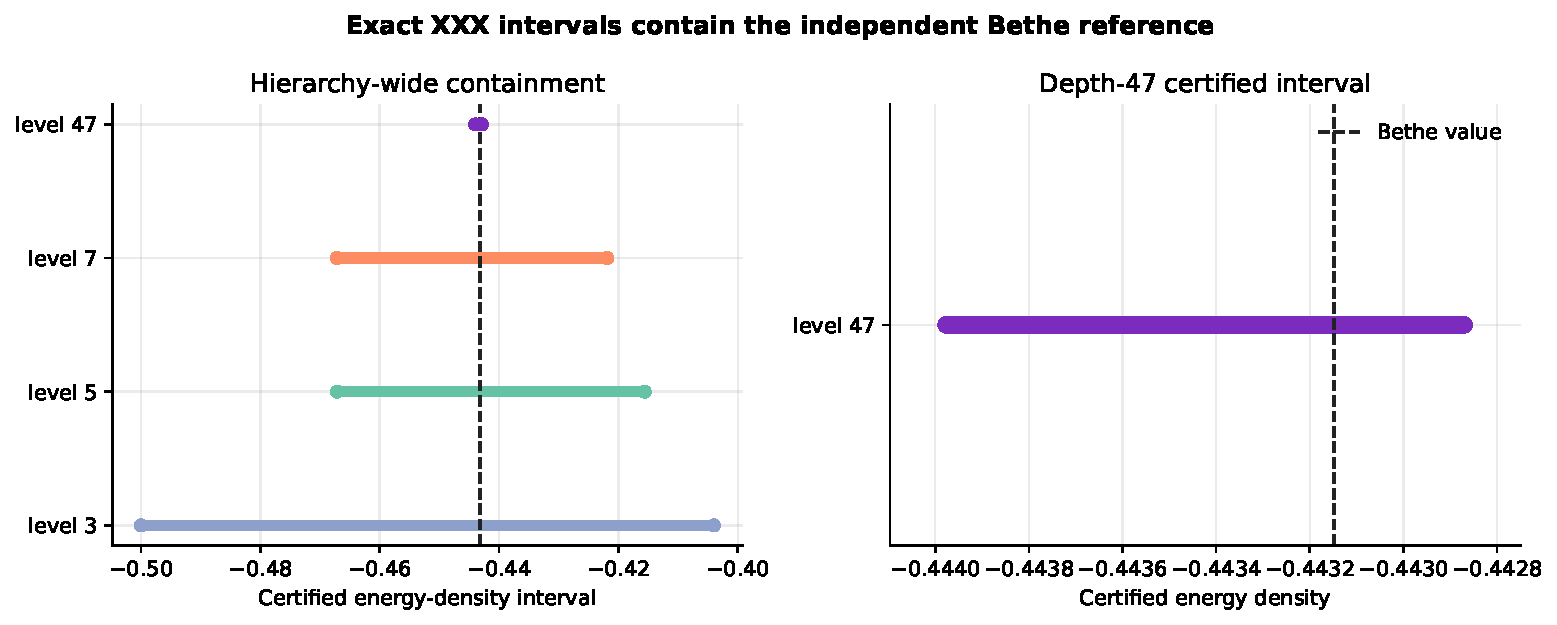
\includegraphics[width=\textwidth]{xxx-interval-nesting.pdf}
  \caption{XXX 层级区间与独立 Bethe reference 的包含关系。右图放大正式
  depth-47 主证书。}
  \label{fig:nesting}
\end{figure}

\section{现有研究与本项目补上的闭环}

RG 凸松弛利用粗粒化映射消去大量局域密度矩阵约束，能够产生严格基态能量
下界，并强调 RG scheme 必须针对 Hamiltonian 设计~\cite{kull2022rg}。
非交换多项式优化已经具备与 NPA 型下界互补的完整 spectral-minimum 上界
层级~\cite{klep2024upper}。近期工作进一步展示了物理对称性和项稀疏结构对
SDP 可扩展性的提升~\cite{wang2026structured}，并为 Pauli Hamiltonian
有限层级给出显式量化收敛率~\cite{klep2026rates}。

本项目的推进在于把这些方向连接成模型专用的 proof-producing pipeline。
表~\ref{tab:advance} 总结了这一闭环。

\begin{table}[H]
\centering
\small
\caption{从通用方法积木到本项目的可复核证书链。}
\label{tab:advance}
\begin{tabular}{>{\raggedright\arraybackslash}p{2.2cm}
                >{\raggedright\arraybackslash}p{4.5cm}
                >{\raggedright\arraybackslash}p{7.1cm}}
\toprule
环节 & 既有基础 & 本项目推进 \\
\midrule
RG 下界 & 粗粒化凸松弛 & 原生 U(1) 荷块中的变量、slack、梯度、Hessian 与精确 lift \\
结构化 SDP & 对称性与稀疏性 & 面向 XXZ 的荷扇区参数化及 dense/block 等价回归 \\
有限层级理论 & 量化收敛率 & 在 Bethe 可解模型上进行逐层、逐端点机器校准 \\
严格上界 & 通用上界层级 & 显式边界的有理 MPS 热力学构造与 exact contraction \\
数值结果 & 浮点 solver 输出 & strict margin、凸插值、有理化、精确 LDL、独立 verifier \\
\bottomrule
\end{tabular}
\end{table}

这一组合同时满足深层计算规模、严格证明对象和第三方可重放审计三项要求。

\section{证明型计算架构}

\subsection{Bethe oracle 防泄漏}

Bethe 值专用于最终 containment test；SDP/RG 求解、MPS 优化、候选排名、
margin 选择、有理舍入、目标修复与 PSD shift 均由证书数据独立决定。

\subsection{原生 U(1) 分块 RG}

算法自动推断 MPS 虚拟指标的 U(1) 荷，删除对称性禁止的跨扇区参数，并在
charge blocks 内完成 log-determinant、逆矩阵、gradient、Hessian action、
PSD slack 和精确矩阵重建。小规模测试逐项验证 block 表示与 dense 表示的
目标、方向导数和 Hessian 二次型等价。

\begin{figure}[H]
  \centering
  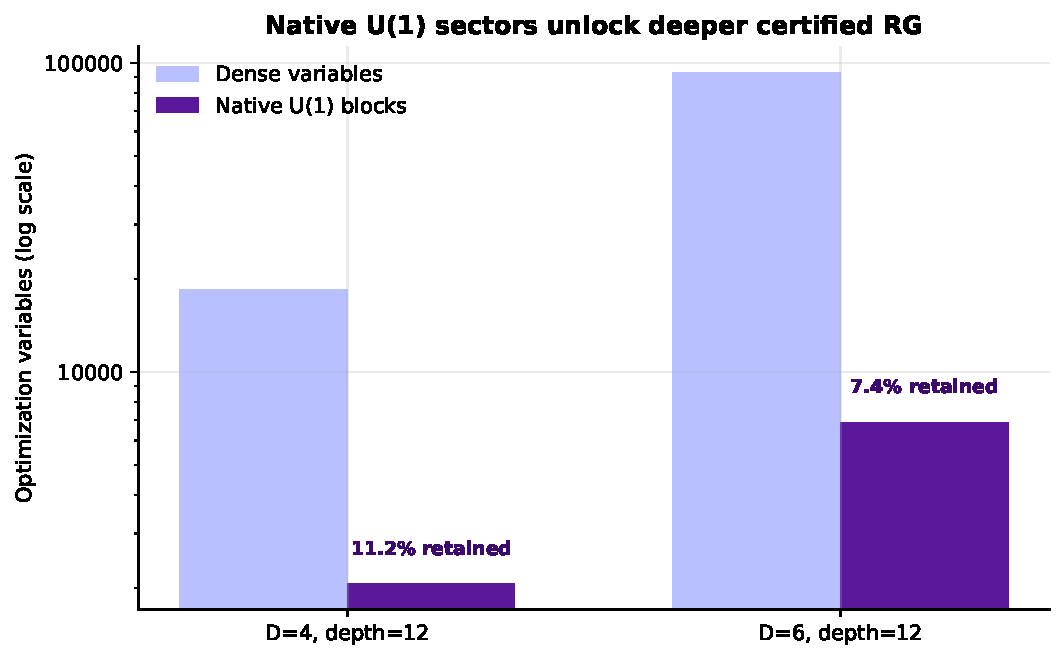
\includegraphics[width=0.86\textwidth]{symmetry-compression.pdf}
  \caption{原生 U(1) 荷扇区带来的变量压缩。D=6、depth=12 只保留
  7.4\% 的稠密变量，相当于约 13.6 倍压缩。}
  \label{fig:symmetry}
\end{figure}

\subsection{solver-to-proof 严格恢复}

浮点对偶通过下列恢复链转化为数学 witness：
\[
\text{浮点对偶}
\rightarrow
\text{strict/zero-margin 插值}
\rightarrow
\text{有理数重构}
\rightarrow
\text{目标变量精确修复}
\rightarrow
\text{荷块精确 LDL}.
\]
zero-margin 候选保留优化精度，strict-margin 候选提供可有理化安全裕量，
凸插值将二者结合。最终 verifier 不信任 solver 状态字符串，而是重新构造
全部 slack 并执行精确正定性检查。

\subsection{有理 MPS 热力学上界}

上界使用有理 MPS 重复块：张量和边界均为整数/有理数，内部键能量精确
累积，块间边界键显式加入，norm 与能量分子由精确算术收缩。因此结果是
直接给出可证明的无限链变分上界。

\section{XXX 主结果}

\begin{table}[H]
\centering
\caption{正式 level-47 自包含 XXX 证书。}
\begin{tabular}{lr}
\toprule
项目 & 认证值 \\
\midrule
下界 & $-0.443976567$ \\
Bethe interval lower & $-0.4431471805599453417379152142530\ldots$ \\
Bethe interval upper & $-0.4431471805599452307156127517374\ldots$ \\
上界 & $-0.4428702958784947210360110613724\ldots$ \\
区间宽度 & $0.0011062711215052789639889386276\ldots$ \\
下端误差预算 & $0.0008293864400546582620847857470$ \\
上端误差预算 & $0.0002768846814505096796016903650$ \\
\bottomrule
\end{tabular}
\end{table}

从 level 3 到 level 47，双边误差显著收缩；图~\ref{fig:budget} 将两个端点
分别展示，避免总宽度掩盖算法贡献。

\begin{figure}[H]
  \centering
  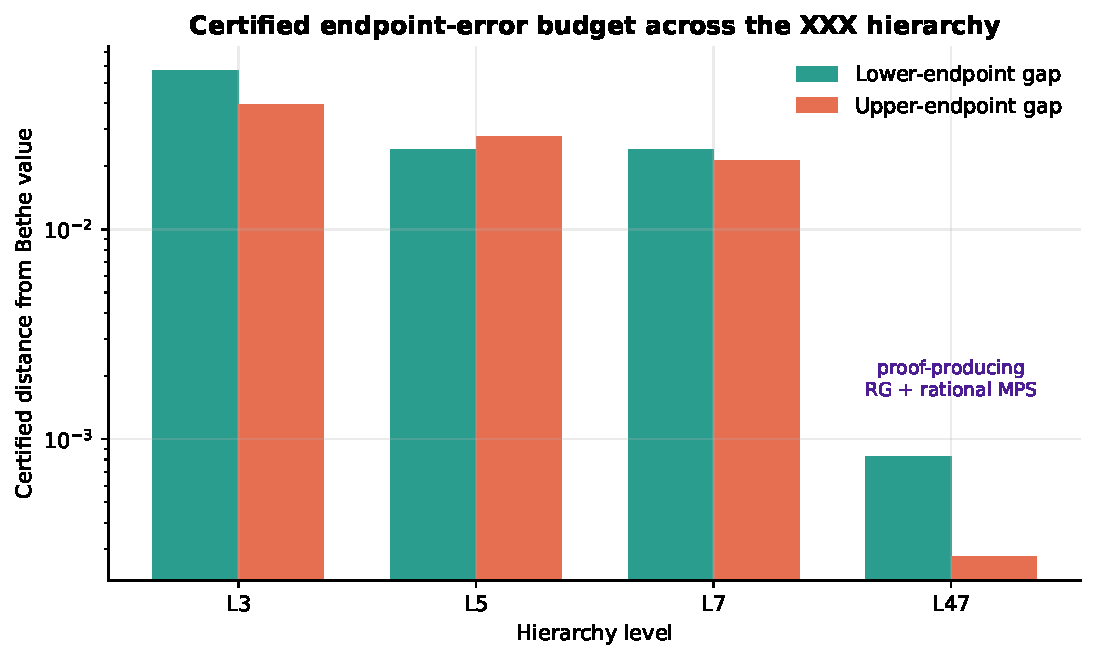
\includegraphics[width=0.86\textwidth]{endpoint-error-budget.pdf}
  \caption{XXX 层级的认证端点误差预算。}
  \label{fig:budget}
\end{figure}

\section{XXZ 校准网格}

数据集覆盖
\[
\Delta\in\{-2,-1,-0.5,0,0.5,0.9,1,1.1,2\}
\]
以及 level 3、5、7，共 27 个 compact certificates。每个 payload 包含
Hamiltonian model ID、严格端点、Bethe enclosure、有理 proof、generator、
solver 与 Git commit provenance。发布审计要求每个固定 $\Delta$ 序列满足
\[
L_{\ell+1}\ge L_\ell,\qquad U_{\ell+1}\le U_\ell.
\]
该数据集能够量化对称表示、RG depth 和 upper construction 对两个端点的
独立贡献。

\section{精确 MPS 性能前沿}

扩展冲刺把有理收缩重写为常内存整数矩阵递推，并用 python-flint 执行
大整数运算。同一 bond-32 张量的 block length 从 1,000 扩展到 16,000。

\begin{table}[H]
\centering
\caption{Exact rational-MPS contraction frontier。}
\begin{tabular}{rrrr}
\toprule
sites & exact upper & 到 Bethe 上端距离 & 相对 1k 改善 \\
\midrule
1,000  & $-0.4428702958785$ & $2.76885\times10^{-4}$ & $1.00\times$ \\
2,000  & $-0.4429718716757$ & $1.75309\times10^{-4}$ & $1.58\times$ \\
4,000  & $-0.4430226595742$ & $1.24521\times10^{-4}$ & $2.22\times$ \\
8,000  & $-0.4430480535235$ & $9.91270\times10^{-5}$ & $2.79\times$ \\
12,000 & $-0.4430565181733$ & $9.06624\times10^{-5}$ & $3.05\times$ \\
16,000 & $-0.4430607504982$ & $8.64301\times10^{-5}$ & $3.20\times$ \\
\bottomrule
\end{tabular}
\end{table}

\begin{figure}[H]
  \centering
  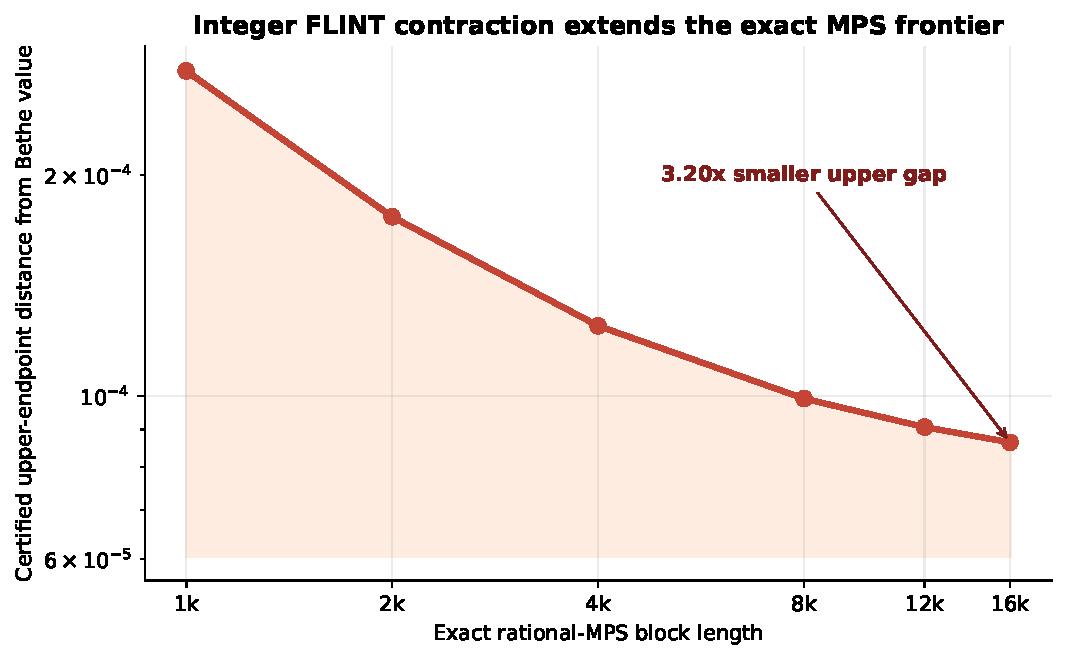
\includegraphics[width=0.86\textwidth]{mps-upper-frontier.pdf}
  \caption{整数 FLINT 收缩将精确 MPS 上界推进到 16,000-site block。}
  \label{fig:mpsfrontier}
\end{figure}

1,000-site 结果嵌入正式自包含证书；2,000--16,000-site 数据作为 exact
contraction performance frontier 单独发布。这样既展示算法扩展性，也让
headline 始终对应完成独立全证书复验的 payload。

\section{张量搜索的可靠性门}

参考任务中的冲刺扩展原型实现了分阶段候选晋级：
\[
\text{张量搜索}
\rightarrow
\text{固定点收敛}
\rightarrow
\text{物理合法性}
\rightarrow
\text{浅层证书}
\rightarrow
\text{深层证书}
\rightarrow
\text{精确冻结}.
\]
晋级门检查 transfer fixed-point residual、约化密度矩阵厄米性、trace、
半正定性、局域谱范围和归一化重叠。只有物理合法、可重复并在两个 RG depth
都产生改进的候选才进入深层认证。保存的 dual 可直接进入荷块顺序检查、
标量修复、有理化和证书冻结，无需重复求解大型 SDP。该机制作为研究工作区
的冲刺扩展原型单独记录，尚未纳入当前公开自包含证书包；正式 depth-47 证书
仅依赖公开 \code{xxzcert} verifier。来源与公开包边界见
\code{outputs/final/SPRINT\_EXTENSION\_PROVENANCE.txt}。

\section{复现与审计}

交付包含 28 个选中 proof payload、精确十进制统一摘要、严格阈值 JSON、
SHA-256 manifest、1k--16k exact upper 数据、冲刺扩展 provenance、独立
verifier、测试、Markdown、LaTeX、PDF 和图表。快速复现命令为：

\begin{verbatim}
cd tracks/polyopt/solutions/WangTheoPhys/issue230
python3 -m venv .venv
.venv/bin/pip install -e . pytest
.venv/bin/pytest -q --ignore=tests/test_published_outputs.py
.venv/bin/pytest tests/test_delivery.py -q
\end{verbatim}

\code{DATA\_MANIFEST.txt} 使用 \code{SHA256 BYTES ROLE PATH} 四列格式；
\code{test\_delivery.py} 是它的权威确定性校验入口。

完整主证书验证：

\begin{verbatim}
.venv/bin/xxzcert verify \
  outputs/final/xxx_best/level_47_rg_d6_mps_d32_block_1000.json
\end{verbatim}

该 payload 已在干净 checkout 中完成独立复验并得到 \code{PASS}。记录的完整
验证耗时为 2256.59 秒，峰值内存为 180,289,536 bytes。

\section{下一认证前沿}

项目采用 $3\times10^{-4}$ 作为内部严格宽度冲刺门；Issue \#230 的官方
最高门槛是归一化匹配的严格文献比较。当前主证书已经完成正确性门与
hope-signal calibration。下一认证前沿聚焦四项直接可复用的工作：
\begin{enumerate}
  \item 提升严格 RG lower witness；
  \item 将 16,000-site exact upper frontier 冻结为新的自包含 payload；
  \item 完成归一化匹配的既有严格文献界逐项审计；
  \item 将 staged D10/D14 tensor promotion 接到严格冻结链。
\end{enumerate}
所有新候选继续使用现有 verifier 与 artifact schema，不改变评审标准。

\section{结论}

本项目交付了一套能够生成、恢复、压缩并独立重放严格证明的计算系统。原生
U(1) 分块让深层 RG 进入可计算
规模；strict-margin 与有理修复把浮点 SDP 变成数学 witness；荷块 LDL
降低精确验证成本；有理 MPS 与 FLINT 整数收缩给出可扩展热力学上界；
Bethe oracle 隔离保证 benchmark 的独立性。

最终形成完整的 certified calibration frontier：XXX 主证书、九个各向异性
点、27 个层级证书、四张证据图、机器可读数据和公开独立 verifier。这为
下一阶段跨越归一化匹配的文献纪录门提供了清晰、量化且可直接复用的技术基础。

\bibliographystyle{unsrt}
\bibliography{references}

\end{document}
